\section{Diskussion}
\label{sec:Diskussion}

Andere einstellungen als in der Anleitung

Die Untersuchung des Selektivverstärkers wurde durch den Sinusgenerator erschwert.
Bei jedem Versuch die Frequenz zu ändern, sprang der Sinusgenerator durch den ganzen Frequenzbereich.
Das Ablesen am AC-Millivoltmeter stellte sich genau so schwierig dar, da der Zeiger sich oft durch die ganze Skala frei bewegte.
Dadurch konnten weder klein- noch großschrittige Untersuchungen vorgenommen werden.
Es wurden Messpaare aufgenommen, die über einen kleinen Zeitraum stabil wirkten.
Teilweise wurden auch verschiedene Spannungen bei denselben Frequenzen notiert.
Eine Filterkurve ist nicht zu erkennen, somit sind Aussagen zum Selektivverstärker schwer zu treffen.

Die Stoffe $\ce{Dy2O3}$ und $\ce{Gd2O3}$ wurden verwendet, da die Messungen vor und nach dem Einführen der Probe sichtbare Differenzen haben.
Es sind große Abweichungen bei den ermittelten Werten und den Theoriewerten zu sehen, besonders zwischen $\chi_T$ und $\chi_R$.
Hierbei beträgt die Abweichung bei beiden Stoffen um 200\%.
Zwischen $\chi_T$ und $\chi_U$ besteht bei beiden Stoffen jeweils eine Abweichung von ungefähr 95\%.
Diese großen Ungenauigkeiten wurden schon nach der Untersuchung des Selektivverstärkers erwartet.

\section{Anhang}
\label{sec:Anhang}
\begin{figure}
    \centering
    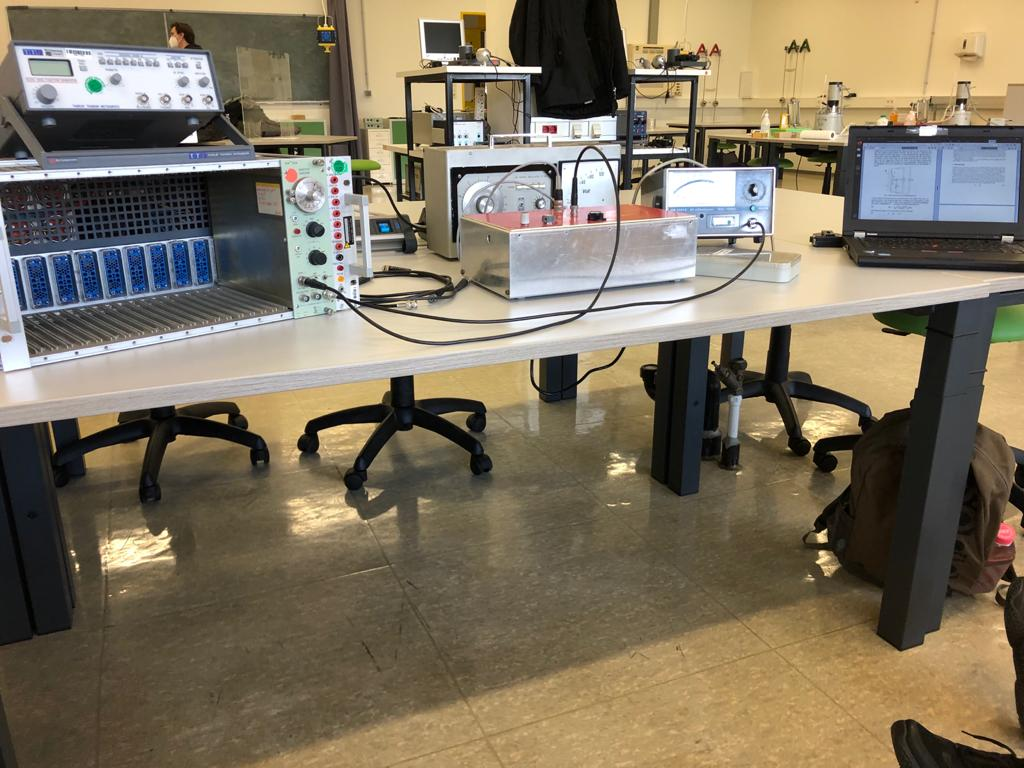
\includegraphics[width=\textwidth]{content/index.jpeg}
    \caption{Das Foto vom Versuchsaufbau.Links im Bild ist der Selektivverstäarker unter einem Sinusgenerator zu sehen. 
    Die Box mit rotem Deckel ist die benutzte Brückenschaltung. 
    Hinter der Brückenschaltung ist der zweite Generator zu erkennen, welcher für die Messung der Suszeptibilität benutzt wurde.
    Rechts außen ist das AC-Millivoltmeter zu sehen.}
    \label{fig:datenselektiv}
\end{figure}
\begin{figure}
    \centering
    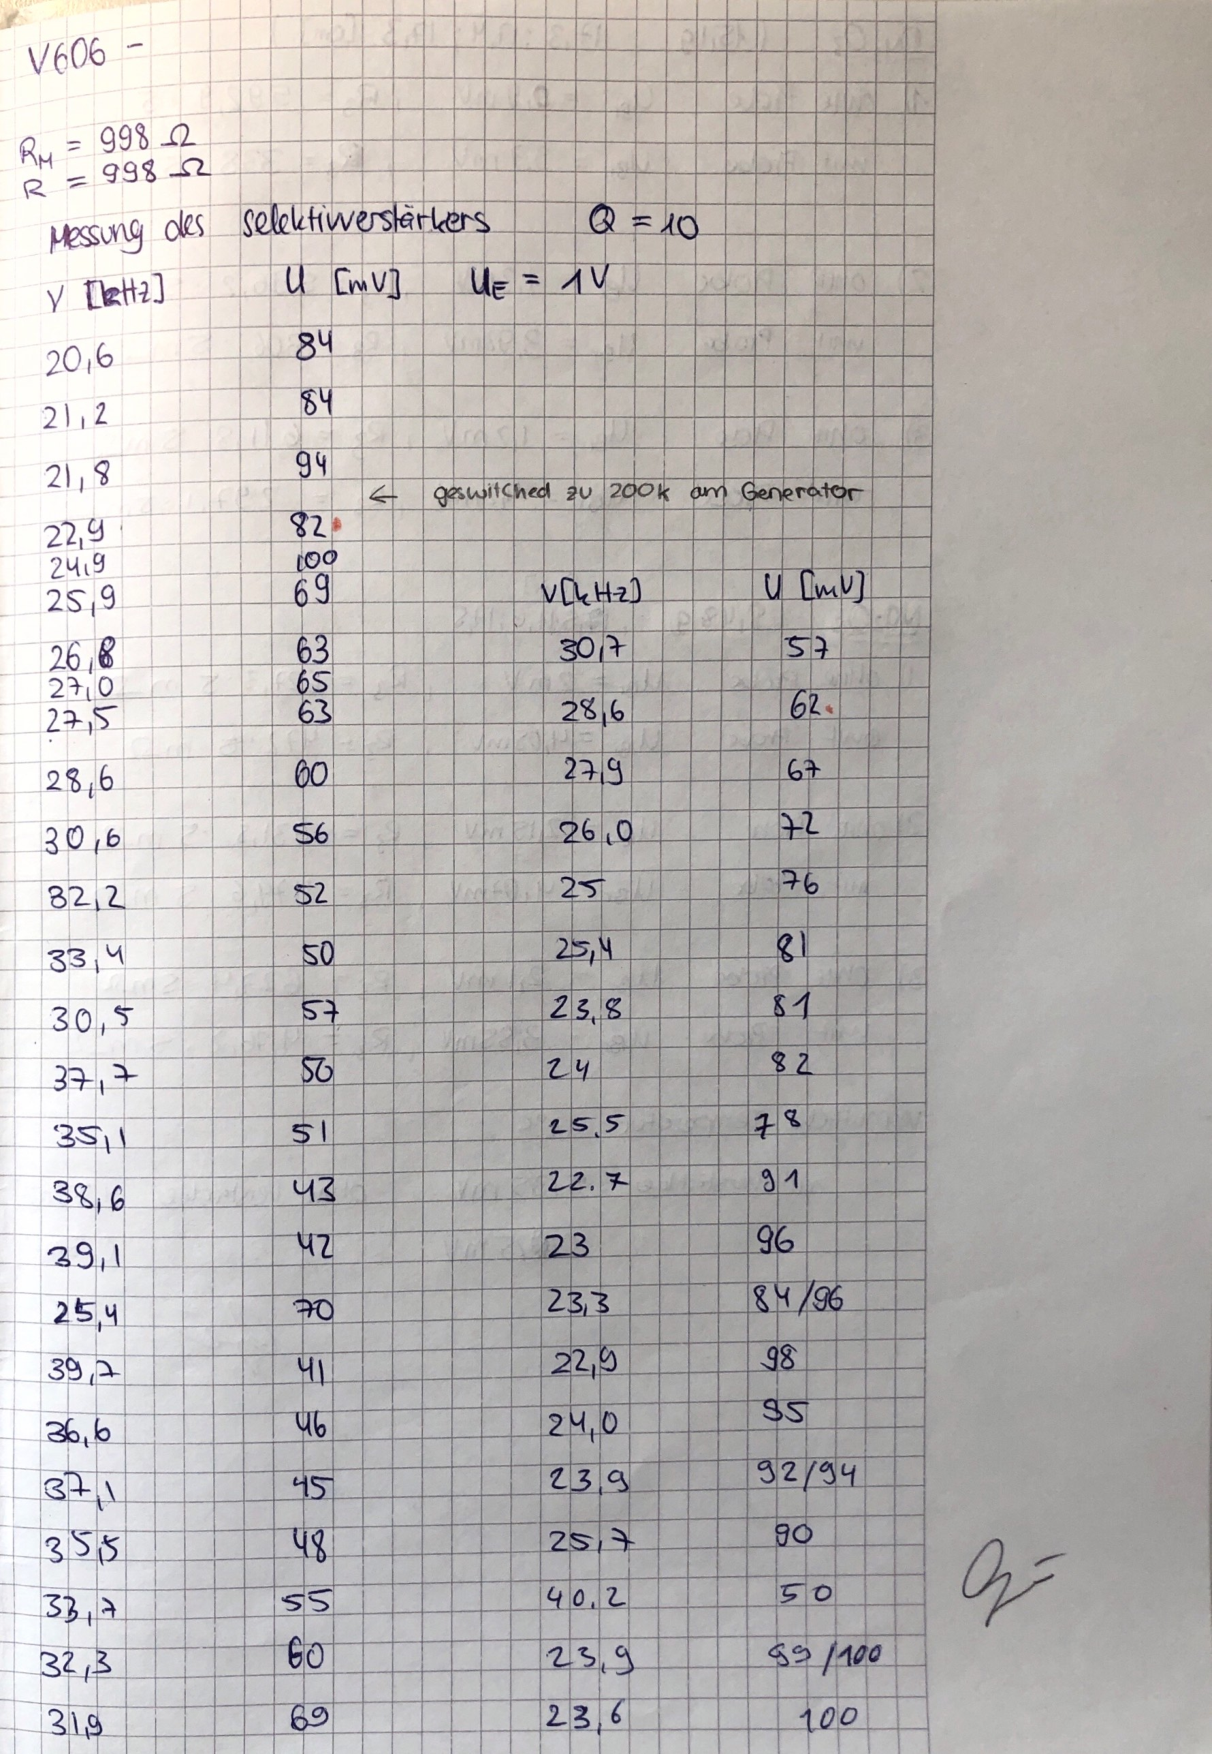
\includegraphics[width=\textwidth]{content/datenselektiv.pdf}
    \caption{Die aufgenommenen Werte für die Messung der Filterkurve des Selektivverstärkers.}
    \label{fig:datenselektiv}
\end{figure}
\begin{figure}
    \centering
    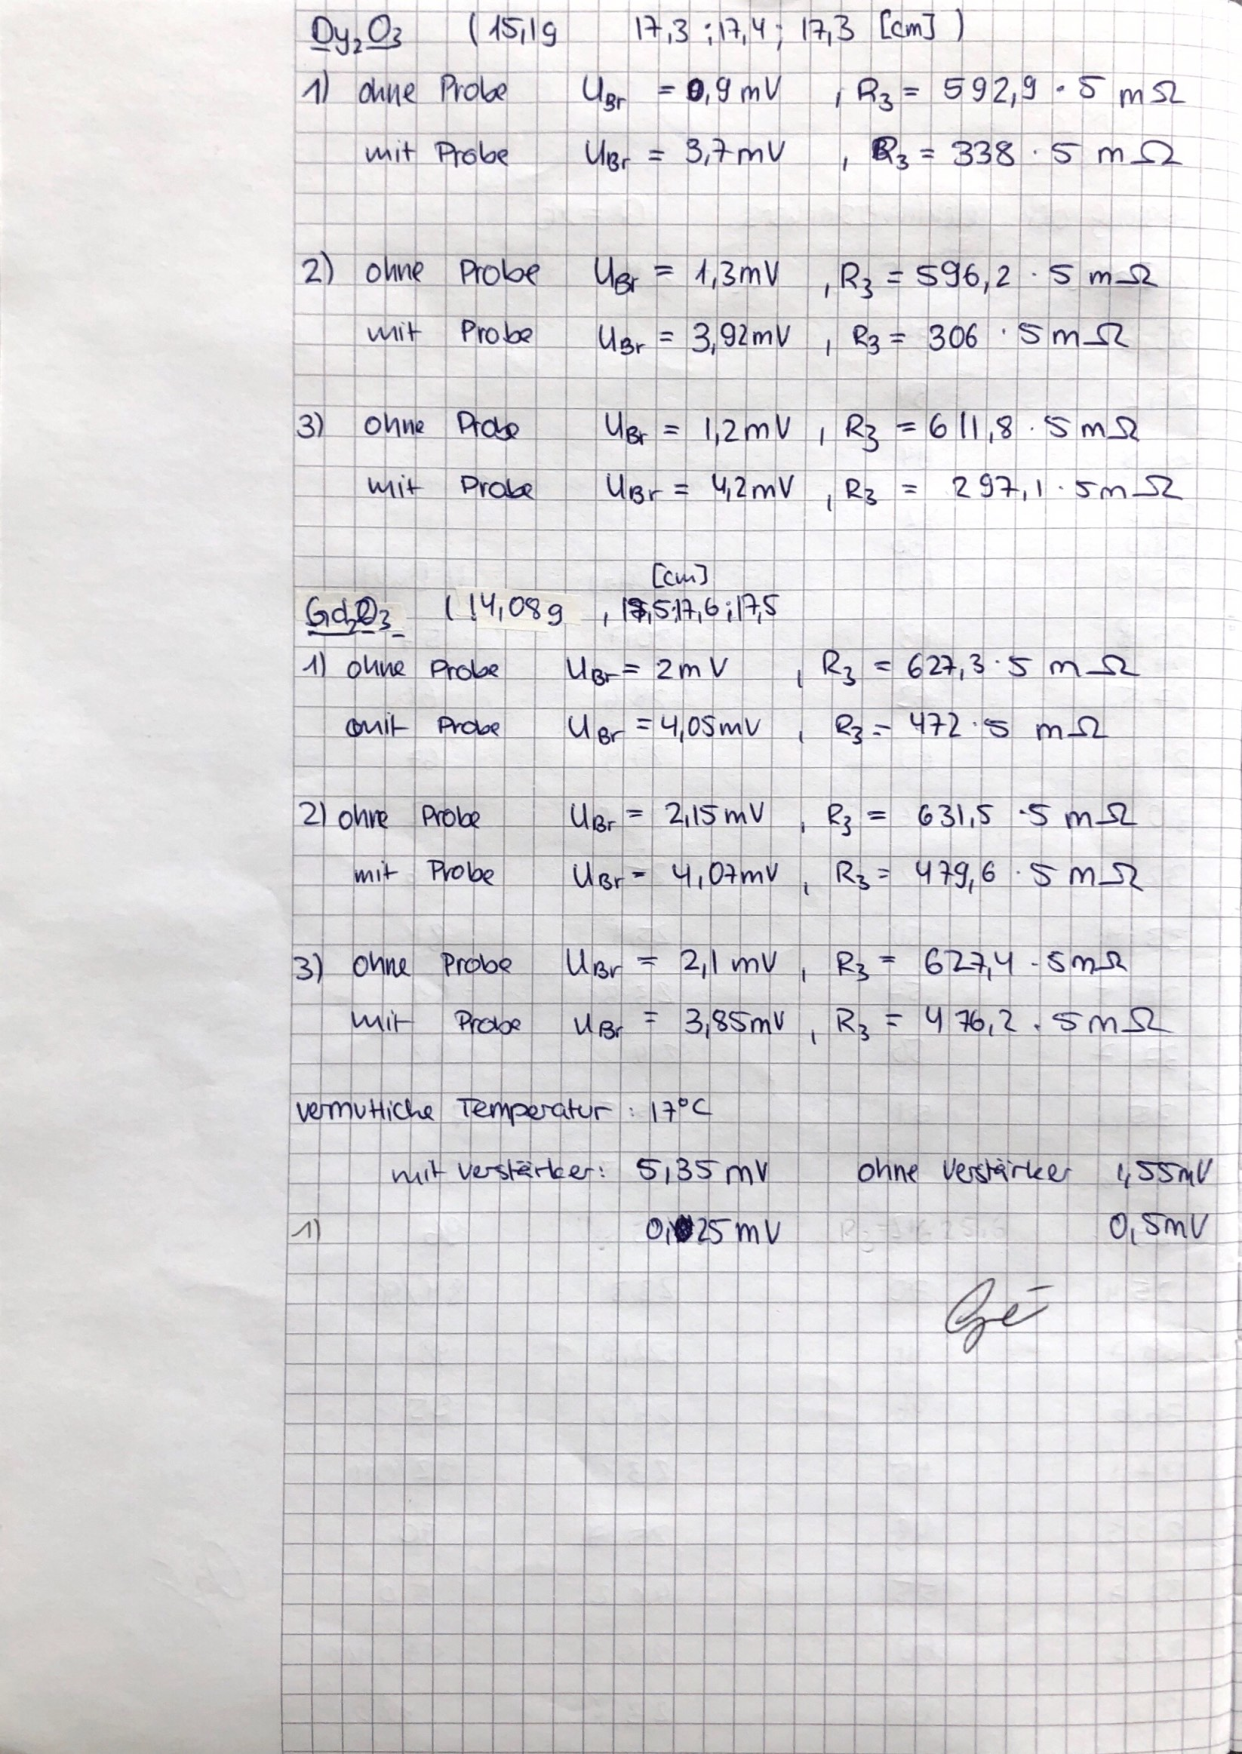
\includegraphics[width=\textwidth]{content/datenmessung.pdf}
    \caption{Die notierten Werte von der Vermessung der paramagnetischen Proben.}
    \label{fig:datenmessung}
\end{figure}
